\begin{task}{3, Training a Variational Autoencoder (VAE) on MNIST}
\paragraph{Implementation} For this task the model is implemented in \verb|vae/model.py|. Also, to make the code more maintainable and modular, the model is trained using another file, \verb|engine.py|, which takes care of running the train and test iterations and providing feedback to the user of the performance measures. In addition, we have support modules such as the visualisation module, the data processing module, or the tool module able to save the weights of the model in a folder. As a user, you should only interact with the \verb|vae.ipynb| notebook to train and test the model.

Our implementation of the VAE is based on the publication \cite{kingma2013auto}. It is composed mainly by an encoder, that approximates the posterior distribution, \(q_\phi (z|x)\), and the decoder that tries to learn the distribution \(p_\theta (x|z)\) in order to learn the latent representation and the underlying distribution of the input data by optimizing the parameters \((\phi, \theta)\). Therefore, apart of trying to learn a correct encoding of the data, we will try to make the approximate posterior distribution to be similar to the assumed distribution of the prior \(p(z)\) by minimising the KL divergence between the two distributions \cite{kullback1951information}.

\begin{figure}[H]
    \centering
    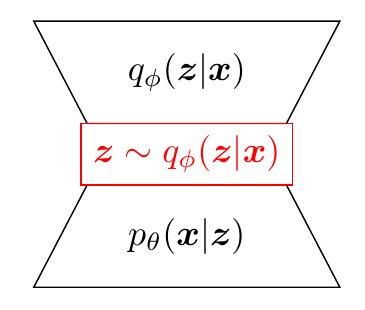
\includegraphics[width=0.4\textwidth]{images/vae.png}
    \caption{Variational Autoencoder structure}
    \label{vaestruct}
\end{figure}

In order to do that, our Variational Encoder outputs the mean \(\mu_e\) and standard deviation \(\sigma_e\) of the approximate posterior, while our Variational Decoder outputs the mean \(\mu_d\) of \(p_\theta (x|z)\), while the standard deviation \(\sigma_d\) is computed as a trainable parameter inside the model. Finally, the VAE model outputs the multivariate diagonal Gaussian distribution of \(p_\theta (x|z)\), using \(\mu_d\) as mean and the diagonalized \(\sigma_d^2\) as covariance matrix, and the mean \(\mu_e\) and the covariance matrix using \(\sigma_e^2\) for \(q_\phi (z|x)\) in order to be able to compute the KL divergence in the loss. \(z\) is sampled from the approximate posterior distribution using the pytorch function \verb|rsample|, which is differentiable.

The chosen dataset to test the model is MNIST, a set of images of handwritten numbers. We will try to learn a latent representation of the data which we can reconstruct, while also trying to make the latent representation continuous enough to be able to generate new samples.

\begin{figure}[H]
    \centering
    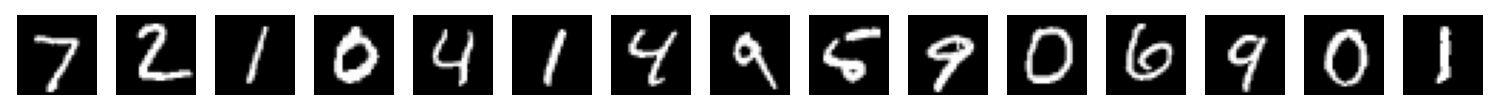
\includegraphics[width=0.9\textwidth]{images/mnist.png}
    \caption{Sample of images of MNIST}
    \label{mnistsample}
\end{figure}

\paragraph{Task 3.1} Regarding the implementation of the encoder and decoder, we needed to choose the activation functions to compute the mean and standard deviation of each distribution. 

For \(\mu_e\) we use a linear activation, as we don't want to impose any constraints on the values of the latent representation. This way allows the encoding to be an unconstrained real number. However, the standard deviation is constrained to be a positive number. Then we apply the exponential function \(e^x\) to obtain \(\sigma_e\).

In the decoder we need to obtain \(\mu_d\) and \(\sigma_d\). Again, the mean is an unconstrained real number. However, we can change its activation function taking into account some external information of the dataset. We are normalizing MNIST pixels to have values between [0,1] so we can constrain \(\mu_d \in [0,1]\) using the sigmoid function (Figure \ref{sigmoid}). Now, the most likely value for a pixel would be already constrained between 0 and 1. On the other hand, the standard deviation for the decoder follows the same rule than in the encoder, therefore we again apply the exponential function to make \(\sigma_d\) always positive.

\begin{figure}[H]
    \centering
    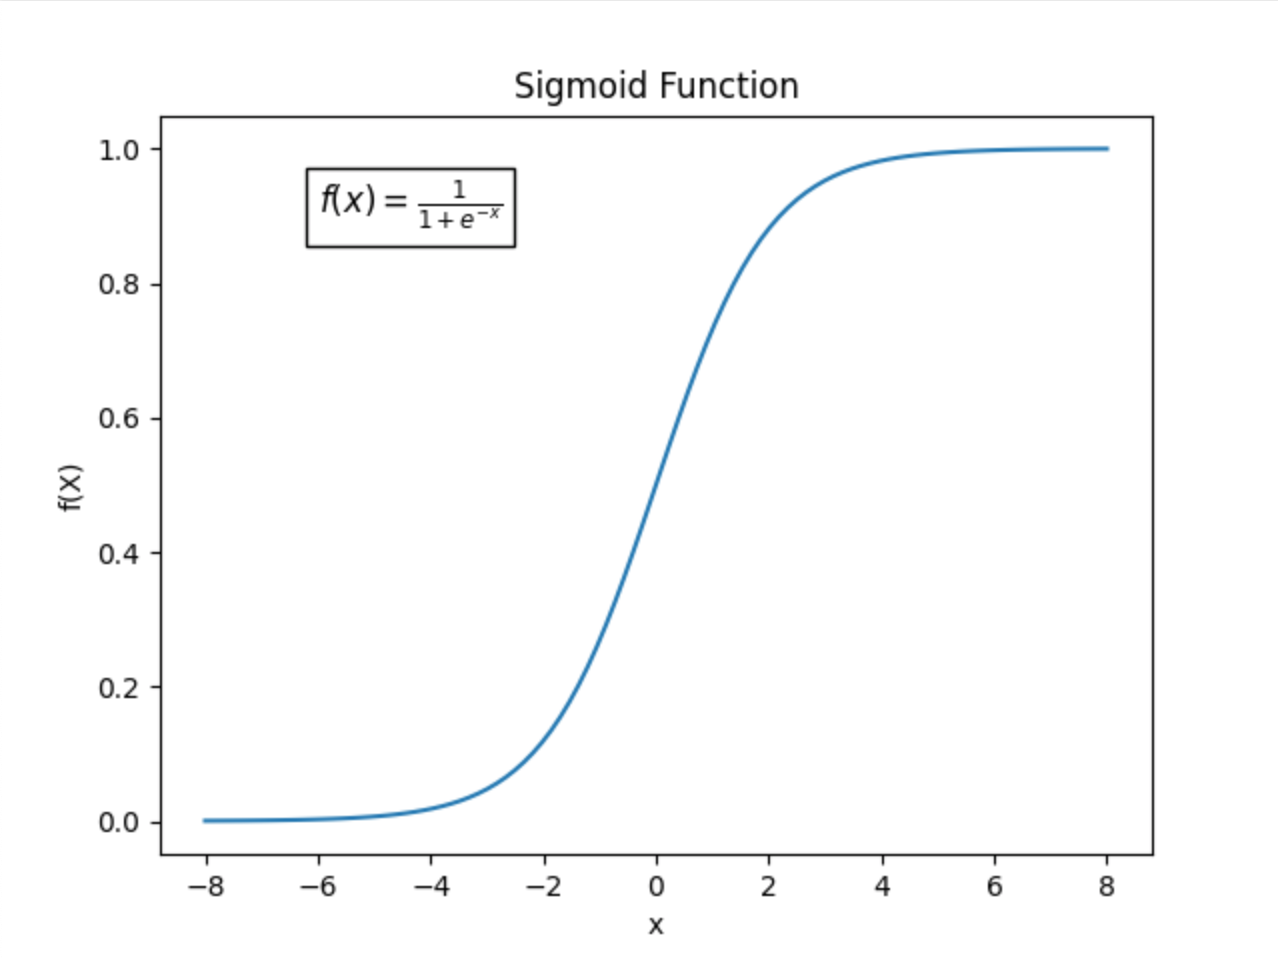
\includegraphics[width=0.5\textwidth]{images/sigmoid-function.png}
    \caption{Sigmoid function}
    \label{sigmoid}
\end{figure}

\paragraph{Task 3.2} We can deduce the cause of obtaining good reconstructed images but bad generated digits. First, we know that the objective function for the VAE is:
\[
\mathcal{L}(x;\phi, \theta) = E_{z\sim q(z|x)}\log p(x|z) - \text{KL}[q(z|x)||p(z)]
\]
The first term controls how similar the distribution of x is given a z-sampled from the approximate \(q(z|x)\). This term encourages the VAE to generate samples from the latent space that can accurately reconstruct the input data. The second term measures how similar are the distribution \(q(z|x)\) from the objective prior distribution \(p(z)\). When the second term is omitted, the VAE acts like an ordinary autoencoder, reconstructing the images from a latent vector z, without applying any constraint to the latent distribution. 

Therefore, we know that the ordinary autoencoders are good at reconstructing and bad at generating due to the latent space distribution being discontinuous, i.e. not being closer to an objective continuous distribution.

Then, we can infer that if our model is bad at generating it is because our latent space is not being properly compressed, i.e. the KL divergence is very high. This means that the approximate posterior is far away from the prior. This can happen when our data is complex and we have too much information to be compressed in the latent space, generating a complex latent distribution. This makes the VAE learn how to reconstruct images but incapable of working with randomly generated samples of latent vectors.

In addition, we can have the opposite problem. Having the KL divergence very low could mean that the distribution \(p(x|z)\) is very similar to the distribution \(p(x)\). This can happen is \(q(z|x)\) ignores \(x\) and returns a \(z\) with 0 mean and unit variance, not compressing information into z and therefore making the decoder to not use the latent vectors for reconstructing. This causes the decoder to reconstruct a blurred image, an average of all the images of the dataset. This is represented in Figure \ref{badkl} as this phenomenon actually happened to us during training. When reaching 20 iterations in an old model the KL loss drastically dropped, making the model reconstruct images as the interpolation of all images of the dataset.

\begin{figure}[H]
    \centering
    \subfigure[Bad reconstructed digits at iteration 25]{
    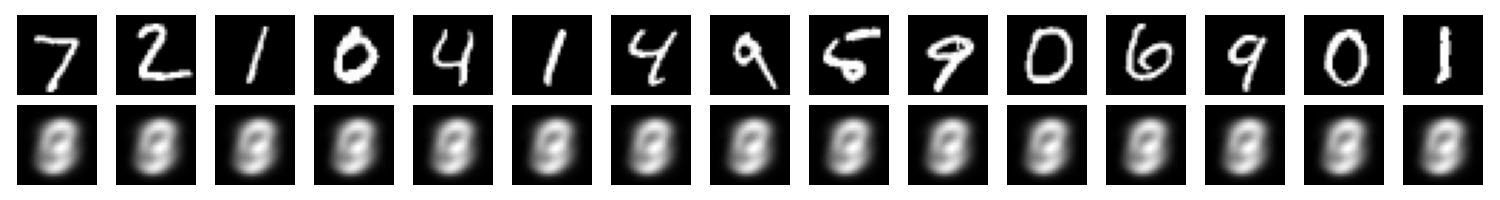
\includegraphics[width=0.9\textwidth]{images/bad_rec.png}}
    \subfigure[Likelihood and KL loss]{
    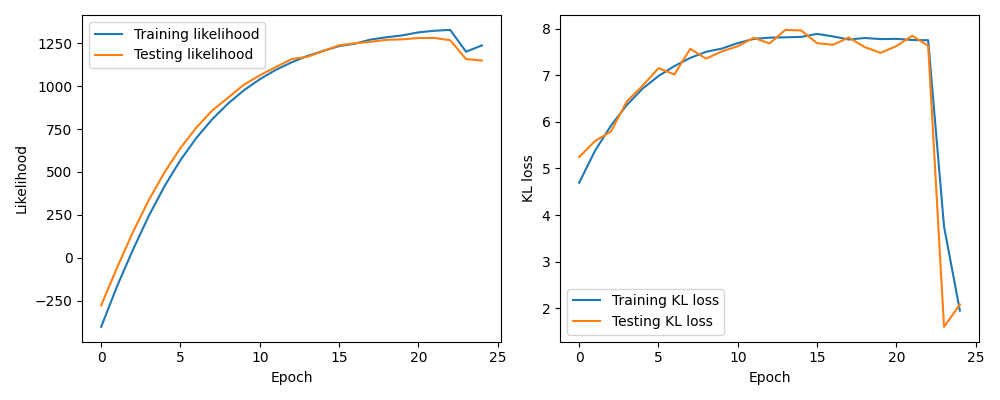
\includegraphics[width=0.6\textwidth]{images/bad_rec_loss.png}}
    \caption{Effects of very low KL divergence}
    \label{badkl}
\end{figure}

\paragraph{Task 3.3} Now, we will test our VAE. We will study how well it reconstructs and generates images at each epoch. We will also study the latent representation structure.

\begin{figure}[H]
    \centering
    \subfigure[MNIST digits]{
    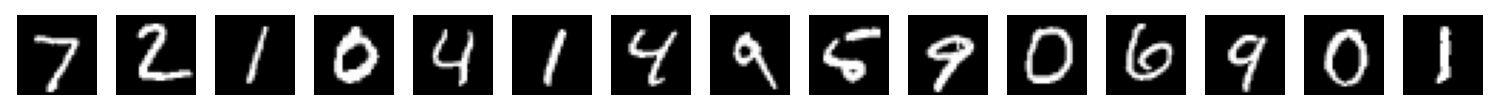
\includegraphics[width=0.9\textwidth]{images/mnist.png}}
    \subfigure[Reconstruction at epoch 0]{
    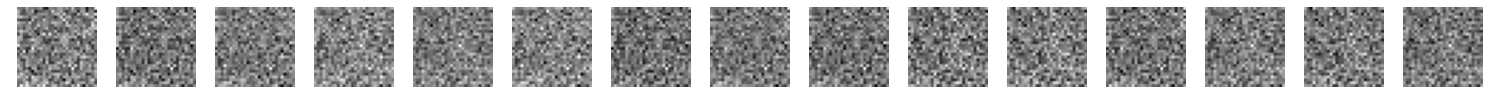
\includegraphics[width=0.9\textwidth]{images/reconstruction_0.png}}
    \subfigure[Reconstruction at epoch 1]{
    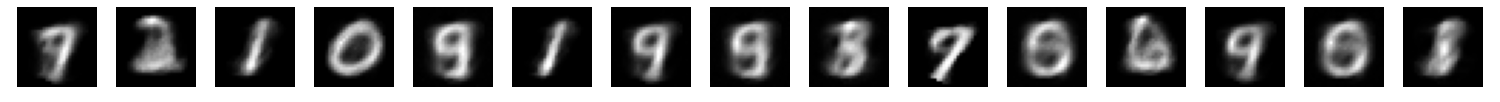
\includegraphics[width=0.9\textwidth]{images/reconstruction_1.png}}
    \subfigure[Reconstruction at epoch 5]{
    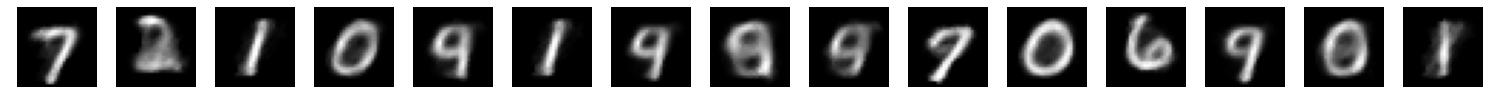
\includegraphics[width=0.9\textwidth]{images/reconstruction_5.png}}
    \subfigure[Reconstruction at epoch 25]{
    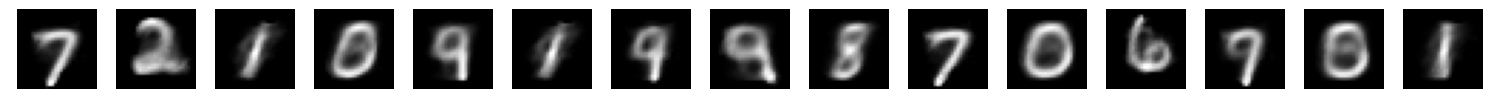
\includegraphics[width=0.9\textwidth]{images/reconstruction_25.png}}
    \subfigure[Reconstruction at epoch 50]{
    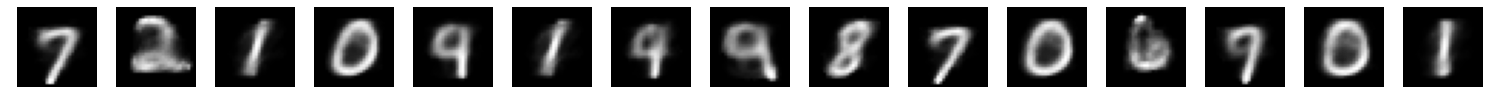
\includegraphics[width=0.9\textwidth]{images/reconstruction_50.png}}
    \caption{Reconstructed images with 2-dimensional latent space}
    \label{rec2d}
\end{figure}

In Figure \ref{rec2d} we can observe how the VAE is reconstructing the same sample of MNIST images. At first the images are a little blurry and some of them seem to be a mixture or interpolation between two or more digits. When reaching 25 epochs all reconstructions are a single digit, without interpolations appearing. Nevertheless, some digits are "mistaken" from others, like the 5 that is reconstructed like an 8, or the two 4 that are reconstructed like 9. This could be related to the encoding of this two numbers being close to the mistaken numbers' encoding. We will explore this later.

\begin{figure}[H]
    \centering
    \subfigure[Generation at epoch 0]{
    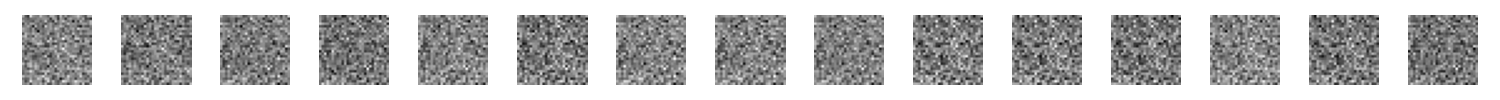
\includegraphics[width=0.9\textwidth]{images/generated_samples_0.png}}
    \subfigure[Generation at epoch 1]{
    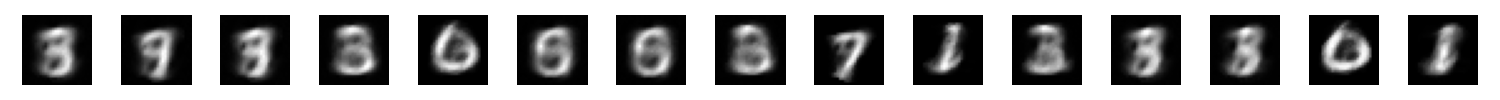
\includegraphics[width=0.9\textwidth]{images/generated_samples_1.png}}
    \subfigure[Generation at epoch 5]{
    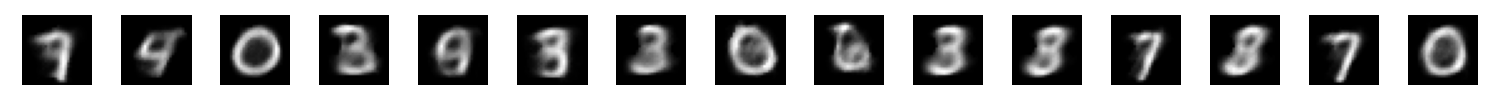
\includegraphics[width=0.9\textwidth]{images/generated_samples_5.png}}
    \subfigure[Generation at epoch 25]{
    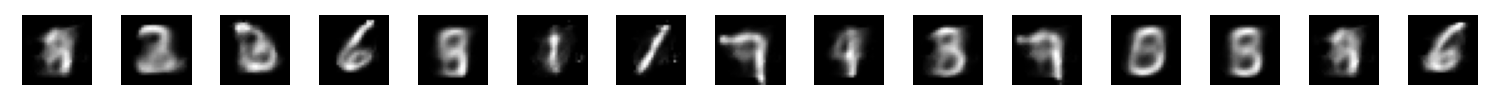
\includegraphics[width=0.9\textwidth]{images/generated_samples_25.png}}
    \subfigure[Generation at epoch 50]{
    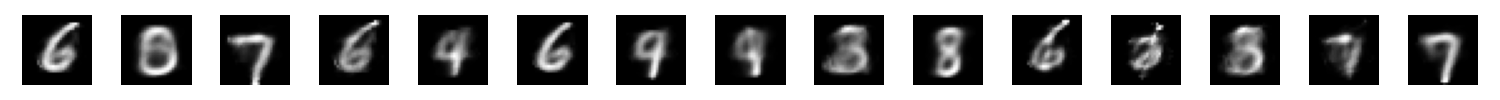
\includegraphics[width=0.9\textwidth]{images/generated_samples_50.png}}
    \caption{Generated images with 2-dimensional latent space}
    \label{gen2d}
\end{figure}

In Figure \ref{gen2d} we can check that our model is better at reconstructing than generating. The generated images are more blurred in the beginning, generating interpolations of digits. After some epochs the model generates clearer digits, however not all of them are perfect. we can see that the digit 6 appears repeatedly, as well as some digits that do not correspond to any real digit.

\begin{figure}[H]
    \centering
    \subfigure[Latent space at epoch 0]{
    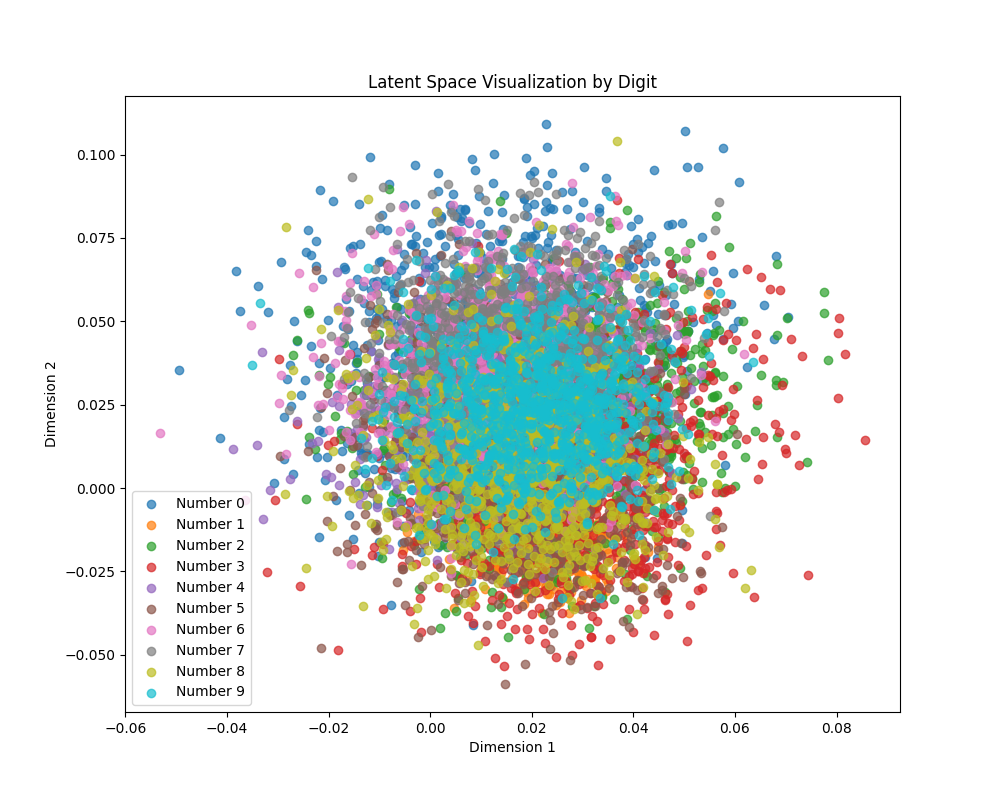
\includegraphics[width=0.45\textwidth]{images/latent_space_0.png}}
    \subfigure[Latent space at epoch 1]{
    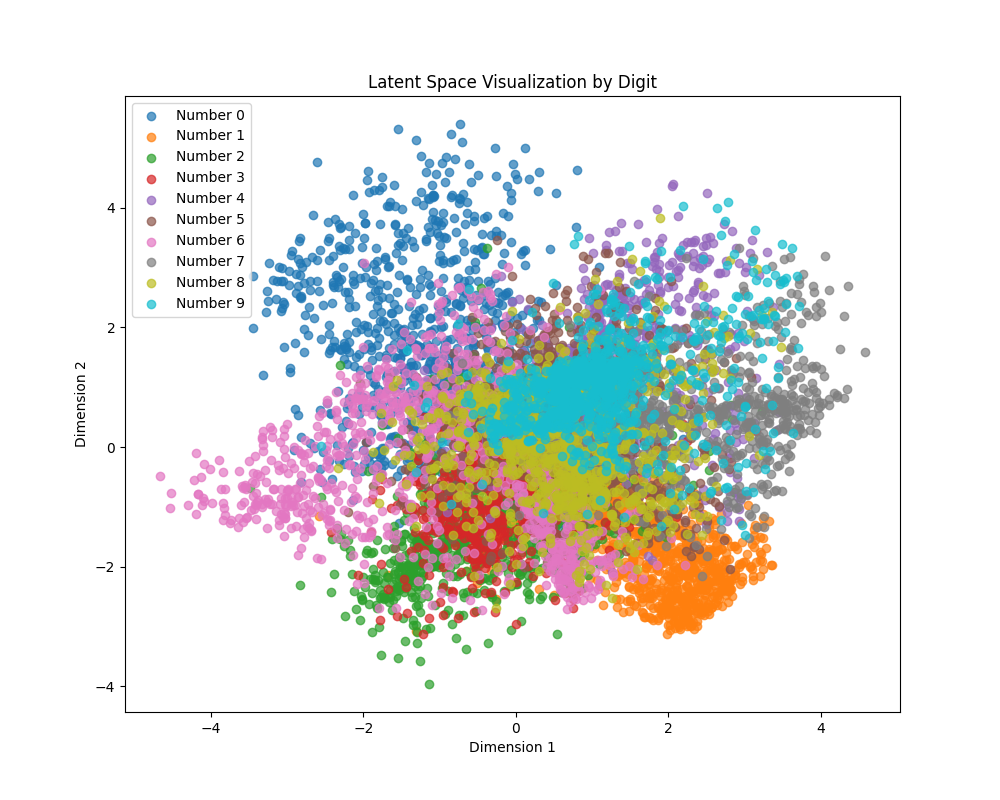
\includegraphics[width=0.45\textwidth]{images/latent_space_1.png}}
    \subfigure[Latent space at epoch 5]{
    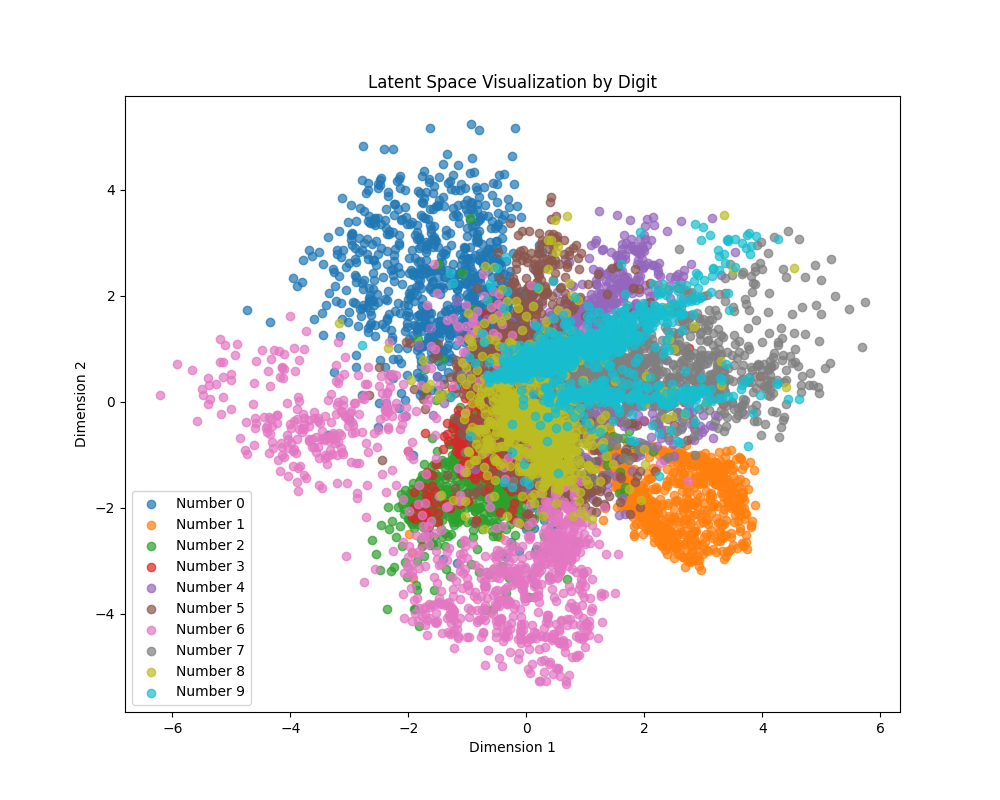
\includegraphics[width=0.45\textwidth]{images/latent_space_5.png}}
    \subfigure[Latent space at epoch 25]{
    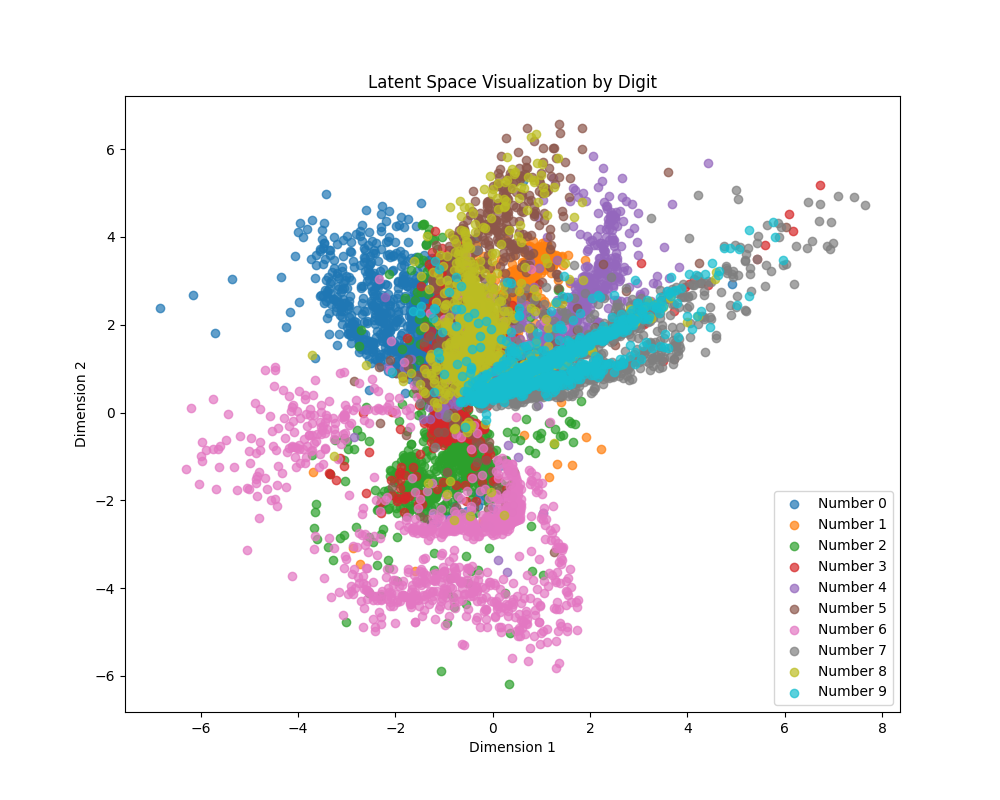
\includegraphics[width=0.45\textwidth]{images/latent_space_25.png}}
    \subfigure[Latent space at epoch 50]{
    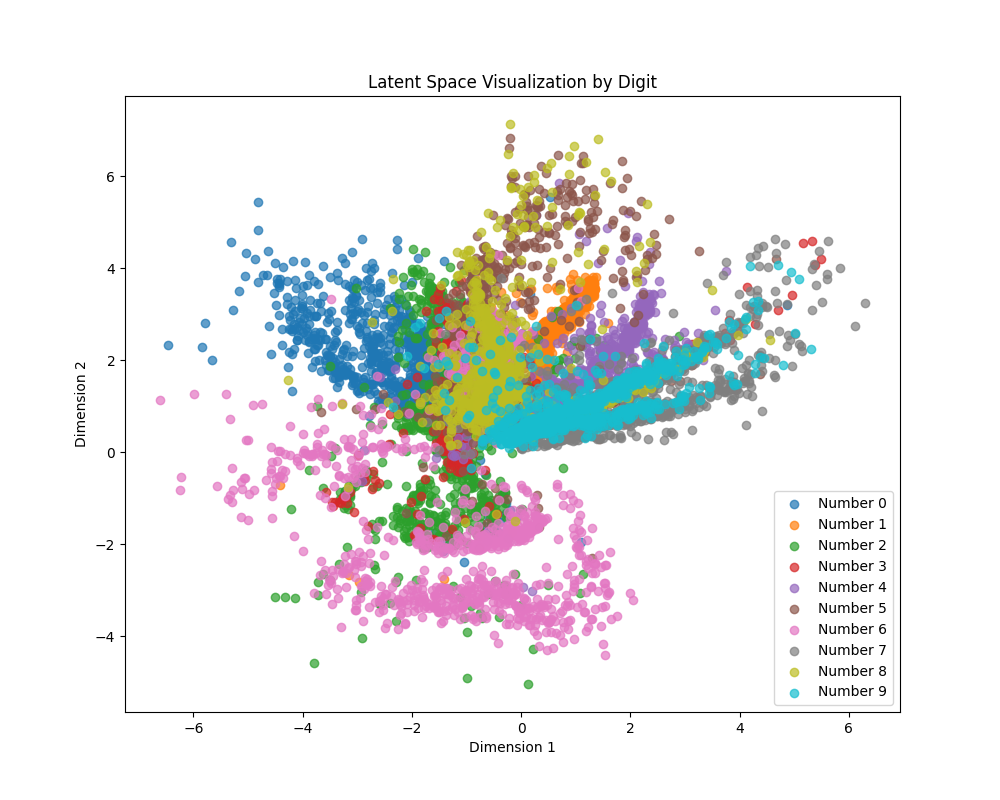
\includegraphics[width=0.45\textwidth]{images/latent_space_50.png}}
    \caption{2-dimensional latent space}
    \label{latent2d}
\end{figure}

In Figure \ref{latent2d} we can observe the evolution of the latent space created by the VAE. At first all the encodings are distributed without an apparent pattern, but quickly thanks to training and the KL regulariser, the latent representations of the different digits start to separate, providing better reconstructions but above all better digit generations, the purpose of VAE. 

Analysing the latent space, we can see how it reflects certain behaviours of our model. For example, the encoding of the number 6 is the most separated and distributed from the rest of the distribution, making the model less likely to be confused in this digit. In this way, we can see how the model properly reconstructs the number 6 in Figure \ref{rec2d} and how it generates it repeatedly in Figure  \ref{gen2d}e, since having the encoding quite spread out makes it more likely that this number will be generated. Another example of this is the number 0, which is usually reconstructed without problems, due to a good encoding that does not overlap with other digits.

On the other hand, we can observe why our model makes mistakes with some digits. For example, it usually mistakes a 4 for a 9 in the reconstruction. If we look closely to Figure \ref{latent2d}d or \ref{latent2d}e, we will notice that the encodings for the digit 4 and 9 are mostly overlapping, making it less likely that the VAE will recover the correct image. 

In summary, we can see how our latent space encodes a distribution that allows us to separate certain digits such as 6 and 0, but suffers with others due to a central area where many latent representations of different numbers overlap.

\paragraph{Task 3.4} Now, we will plot the loss or \(-\mathcal{L_{ELBO}}\). It is important to previously understand that minimizing the \(-\mathcal{L_{ELBO}}\) is equivalent to maximizing the likelihood of the output distribution for the sampled z and minimizing the KL divergence between the approximate posterior and the prior.

\begin{figure}[H]
    \centering
    \subfigure[Loss for 25 epochs]{
    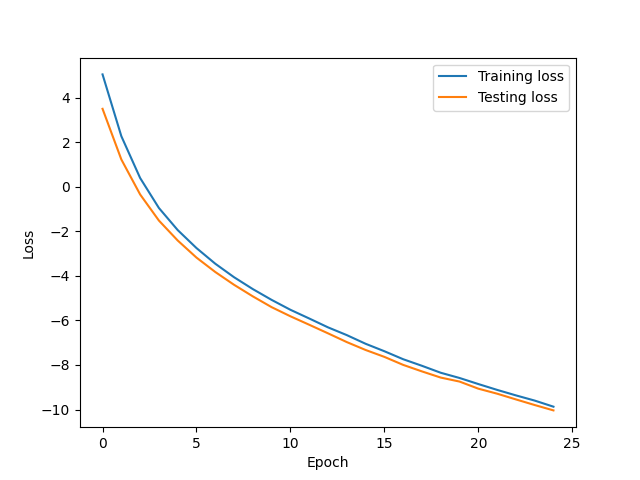
\includegraphics[width=0.45\textwidth]{images/loss_comparison_25.png}}
    \subfigure[Likelihood and KL loss]{
    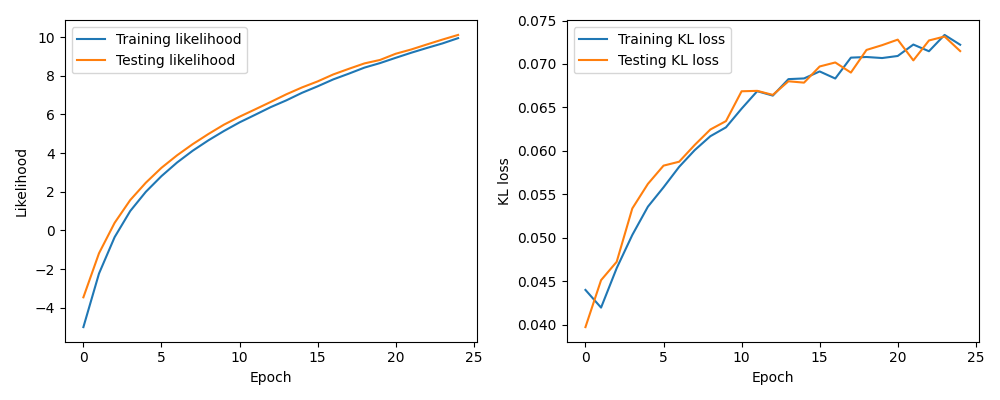
\includegraphics[width=0.6\textwidth]{images/likelihood_and_kl_loss_25.png}}
    \caption{Training and testing loss for 25 epochs}
    \label{loss25}
\end{figure}

In the Figure \ref{loss25} we can observe how the loss is minimized throughout the training, while both the likelihood and the KL loss tend to increase. There are a couple of things that are interesting to note. 

First, we can see how the testing loss is slightly smaller than the training loss, as well as the testing likelihood is slightly greater than the training one. After checking that the inner functioning of the model is correct, we can explain that this could happen because the training and the test data are very similar in MNIST, as it is composed of the same 10 numbers written in a lightly different way, but where the average distribution for each digit should remain. Therefore, the likelihood for training and testing are almost the same, but when this likelihood is subtracted to KL, which is on average higher in testing than in training due to a more random behaviour, produces this small counter-intuitive difference between both losses.

Second, we can observe how the KL loss is increasing instead of reducing, but in a very small magnitude, being almost constant. This can be happening because the actual value of KL is small and the latent encodings need to be less compressed in order to obtain better reconstructions, thus making smaller changes to the latent space sparsity. This can be noted in Figure \ref{latent2d} where the distribution starts with a very clear Gaussian structure and then gradually dissipates. Thus, it seems that the likelihood is the dominant term in the loss function.

Finally, after training the model for 25 epochs more, we can observe how the testing likelihood drastically dropped, while the KL divergence remains almost constant (Figure \ref{loss50}, between 0.071 and 0.075. This could mean that the model is overfitting, being more specialized in the training dataset. 

However, the reconstruction seems to be just as good as the one for 25 epochs. They are almost identical, showing that the model is not improving anymore. Nevertheless, the reconstruction is not bad in spite of having a drop in likelihood. Therefore, we think that this change may not be caused by overfitting but by numerical stability or exploding gradients in the model. 

With more time available, a more in-depth study of the true cause of this strange behaviour could be done, but for the moment we have decided to assume that the model converges around 25 epochs, as the testing loss starts to increase after that.

\begin{figure}[H]
    \centering
    \subfigure[Loss for 25 more epochs]{
    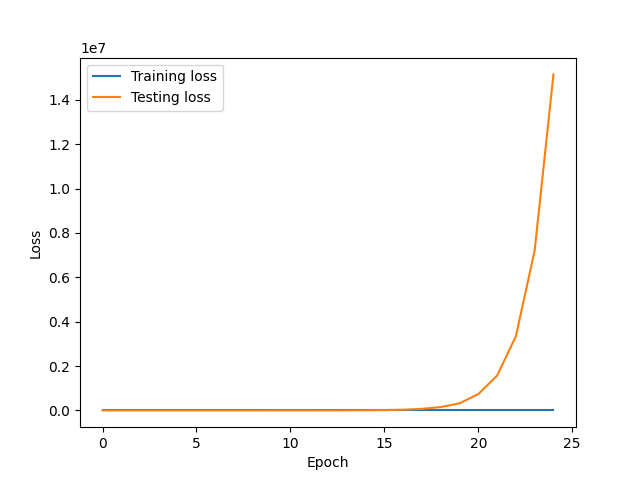
\includegraphics[width=0.45\textwidth]{images/loss_comparison_50.png}}
    \subfigure[Likelihood and KL loss]{
    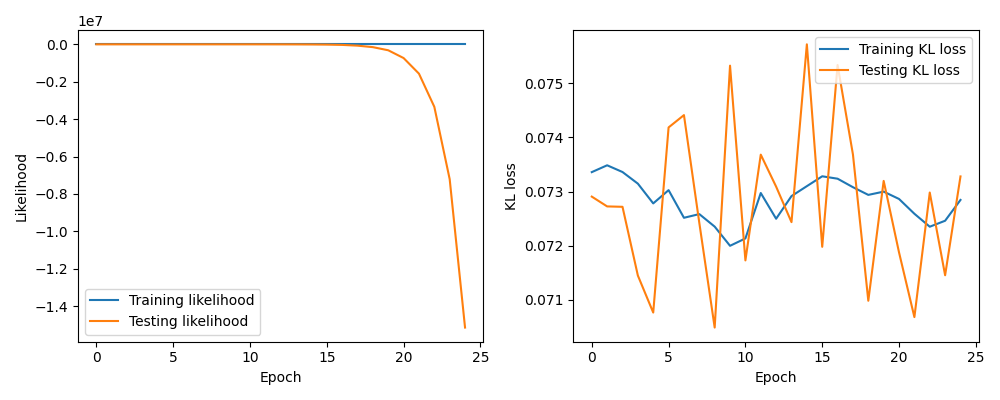
\includegraphics[width=0.6\textwidth]{images/likelihood_and_kl_loss_50.png}}
    \caption{Training and testing loss for 25 more epochs}
    \label{loss50}
\end{figure}

\paragraph{Task 3.5} Now, in order to explore the capabilities of the model with a bigger latent dimension, we have trained and tested the same model of the previous task but changing its latent dimension to 32. 

This time, as we can observe in Figure \ref{rec32d} the reconstruction is almost perfect for the human eye, which sees the whole of the pixels. The reconstruction is far better than the one with a 2-dimensional latent space. We can infer that what causes such accurate reconstructions is a more expressive latent space, i.e. a latent space that allows for the representation of more complex information as it is not as compressed as two-dimensional space. Now, \(z\) can hold more relevant information to be able to reconstruct the images with more accuracy and detail.

\begin{figure}[H]
    \centering
    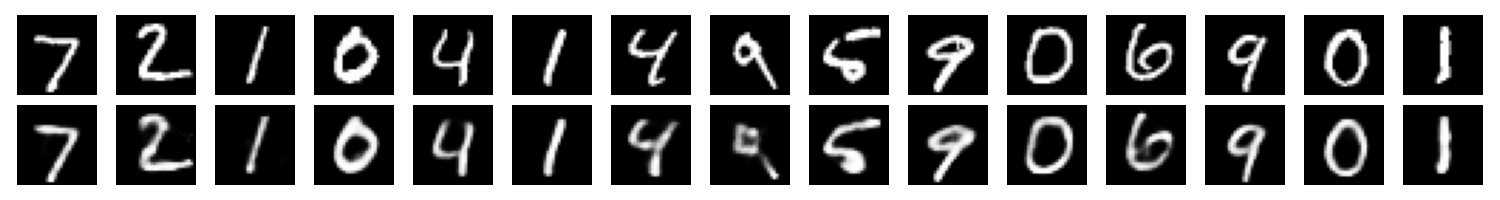
\includegraphics[width=0.9\textwidth]{images/reconstruction_25_32.png}
    \caption{Reconstructed images with 32-dimensional latent space}
    \label{rec32d}
\end{figure}

However, when generating images the model is worse than the one with 2-dimensional space as we can see in Figure \ref{gen32d}. The reason for this may be the same as why we get good reconstructions. A higher dimensional latent space allows for better separation and identification of each number, but makes it more difficult for the model to transform a 32-dimensional random vector into a reasonable image, as there is a higher probability that the random vector is not close to any number distribution.

\begin{figure}[H]
    \centering
    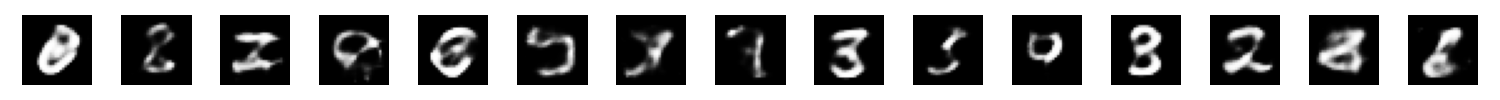
\includegraphics[width=0.9\textwidth]{images/generated_samples_25_32.png}
    \caption{Generated images with 32-dimensional latent space}
    \label{gen32d}
\end{figure}

However, there is an interesting detail that can be noted. There are some numbers that are better generated than others, like the number 3. We wanted to study this phenomenon a little more so we decided to plot the latent space of the model. As it is a 32-dimensional space we needed to transform it into a displayable space, i.e. 2-dimensional or 3-dimensional. 

We selected the UMAP algorithm as it aims to preserve both local and global relationships in which we are more interested \cite{mcinnes2018umap}. Also it is based on manifold theory. Therefore UMAP was more appropriate than t-SNE for the analysis we wanted to do.

In Figure \ref{umap32} we can observe the local and global relationships of the data in lower dimensions. In \ref{umap32}a we can observe how the number 3 distribution seems to be a little further away from the rest of the distributions. This fact is confirmed when the space is shown in 3 dimensions in \ref{umap32}b , which allows us to see how the number 3 is totally separated from the central distribution cloud. This allows that, when the random vector to be generated falls within the distribution of 3, it will be much easier for the model to identify it, generating a clearer picture without traces of interpolations with other numbers.

\begin{figure}[H]
    \centering
    \subfigure[32-dimensional to 2-dimensional space with UMAP]{
    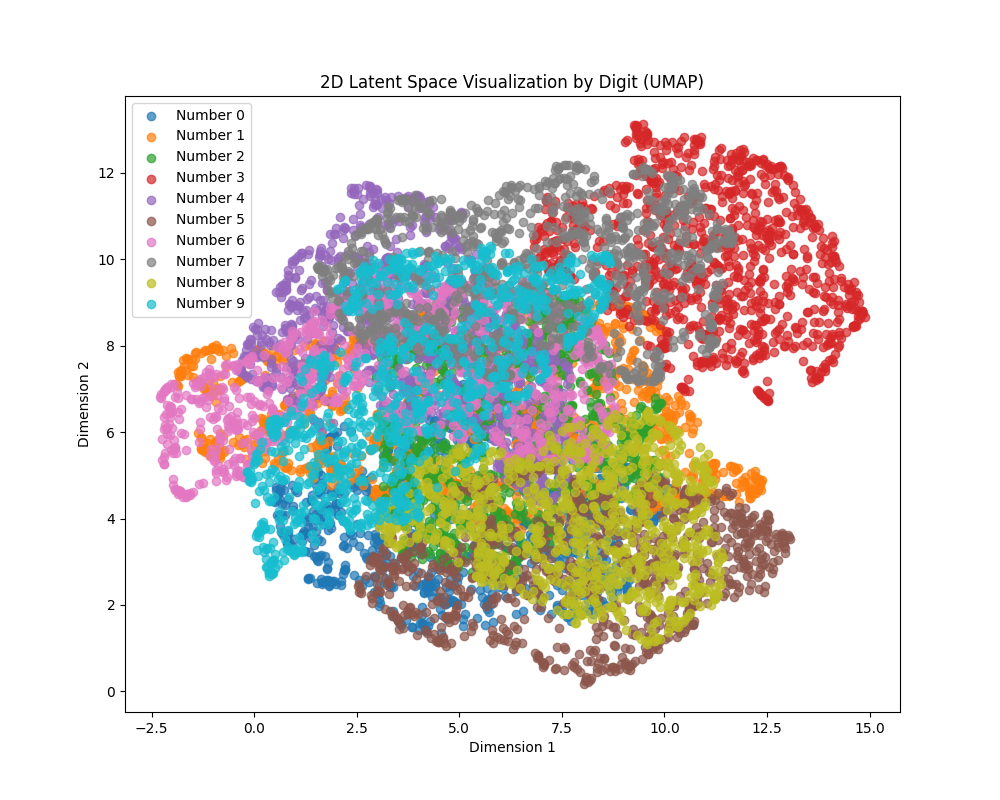
\includegraphics[width=0.6\textwidth]{images/latent_space_umap_25_32.png}}
    \subfigure[32-dimensional to 3-dimensional space with UMAP]{
    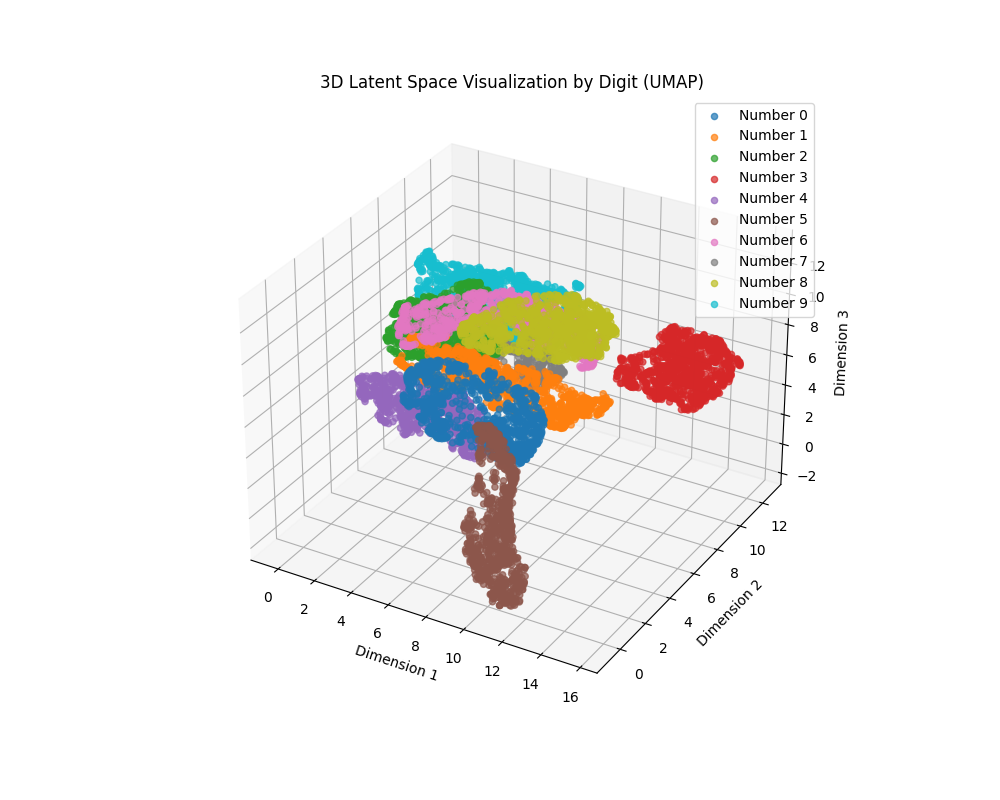
\includegraphics[width=0.7\textwidth]{images/latent_space_umap_3d.png}}
    \caption{32-dimensional space projected into displayable dimensions}
    \label{umap32}
\end{figure}

As we can observe in Figure \ref{loss25_32} the loss evolves in a similar way than for the 2-dimensional model. The loss decreases each epoch, i.e. the likelihood increases at a bigger rate than the kl divergence increases. This indicates that the VAE architecture is easily scalable and that training does not suffer from increasing the dimension of the latent space.


Finally, after the 23 epoch, we can see how the training loss continues to fall while the testing loss remains similar, indicating that the model has reached its point of maximum generalisation. After 25 epochs, something similar to the previous model happened (Figure \ref{loss50}), the testing likelihood explodes and drops drastically, while the training likelihood continues to increase slightly. Therefore, we have used also the model with 25 epoch as the converged model for the 32-dimensional space.


\begin{figure}[H]
    \centering
    \subfigure[Loss for 25  epochs]{
    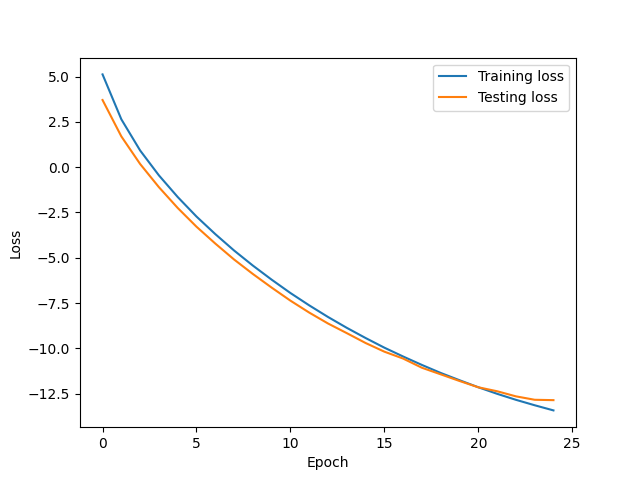
\includegraphics[width=0.45\textwidth]{images/loss_comparison_25_32.png}}
    \subfigure[Likelihood and KL loss]{
    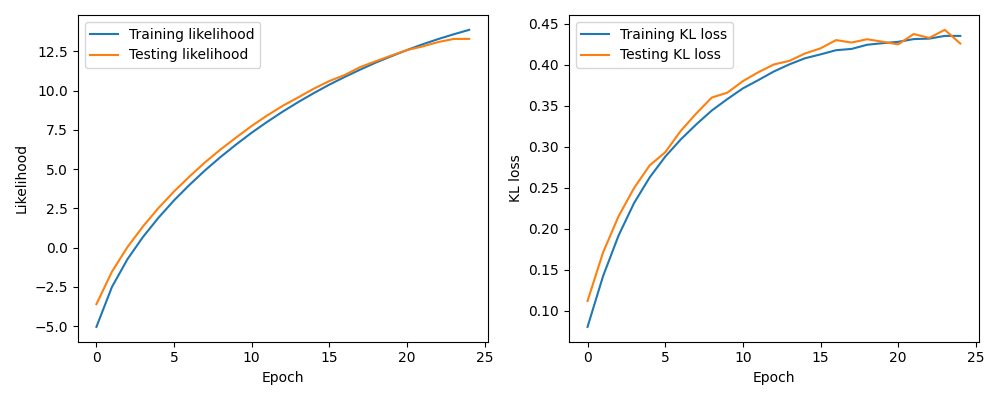
\includegraphics[width=0.6\textwidth]{images/likelihood_and_kl_loss_25_32.png}}
    \caption{Training and testing loss for 25 epochs in 32-dimensional model}
    \label{loss25_32}
\end{figure}

\paragraph{\(\beta\)-VAE implementation} We had achieved a very good reconstruction with the 32-dimensional VAE, however we had not been able to generate digits at the same level. We wanted to try to improve our generation capacity and therefore, based on the  "\(\beta\)-VAE: LEARNING BASIC VISUAL CONCEPTS WITH A CONSTRAINED VARIATIONAL FRAMEWORK" publication \cite{higgins2016beta}, we implemented a \(\beta\)-VAE.

Basically the \(\beta\)-VAE adds a parameter \(\beta\ \in \mathbb{R}\) that controls the strength of the regularizer KL:
\[
\mathcal{L}(x;\phi, \theta) = E_{z\sim q(z|x)}\log p(x|z) - \beta \text{KL}[q(z|x)||p(z)]
\]
Therefore, setting the \(\beta\) to 0 omits the KL divergence, thus converting the VAE in an ordinary autoencoder. Consequently, setting \(\beta\) to values below 1 decreases the importance of KL in the loss function making the latent space distribution less constrained. However, for values greater than one KL will have more regularising strength, resulting in a latent space with a distribution closer to the prior.

As we desired better generations, we wanted the latent space to be more constrained and closer to the prior distribution. Therefore, we did some test with \(\beta > 1\). The most relevant are the following:

\paragraph{\(\beta\) testing for 2-dimensional VAE} We tested different values of \(\beta\) as 10 and 30. We also tested smaller values but the results were very similar to \(\beta = 1\), so we do not include them here.

\begin{figure}[H]
    \centering
    \subfigure[Generated digits with \(\beta = 1\)]{
    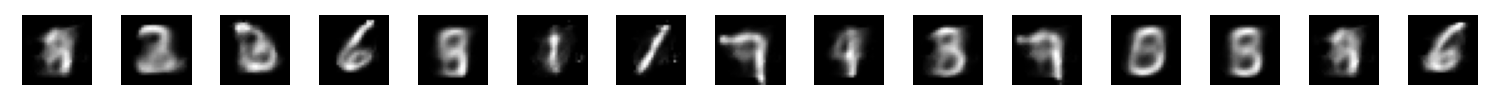
\includegraphics[width=0.9\textwidth]{images/generated_samples_25.png}}
    \subfigure[Generated digits with \(\beta = 10\)]{
    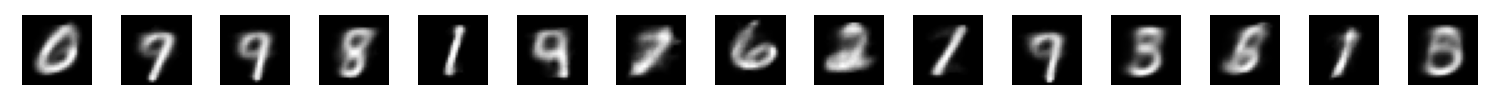
\includegraphics[width=0.9\textwidth]{images/generated_samples_beta10.png}}
    \subfigure[Generated digits with \(\beta = 30\)]{
    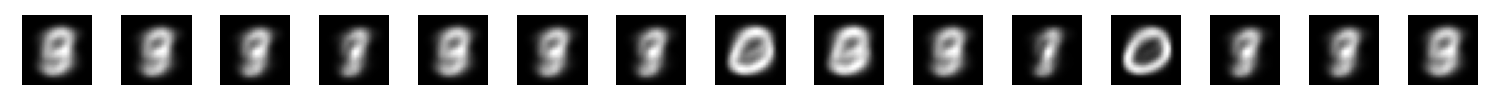
\includegraphics[width=0.9\textwidth]{images/generated_samples_beta30.png}}
    \caption{Comparing generated samples for different \(\beta\) values}
    \label{beta2dgenerated}
\end{figure}

As we can observe in Figure \ref{beta2dgenerated}, after 15 epochs, the results using \(\beta = 10\) have improved the results for generated digits, being them slightly clearer and defined. However, when increasing too much \(\beta\) we can observe how the KL is over regularized, constraining too much the distribution and making the model output an average image. We can further deepen the results by looking at the structure of the latent space.

\begin{figure}[H]
    \centering
    \subfigure[Latent space for \(\beta = 10\)]{
    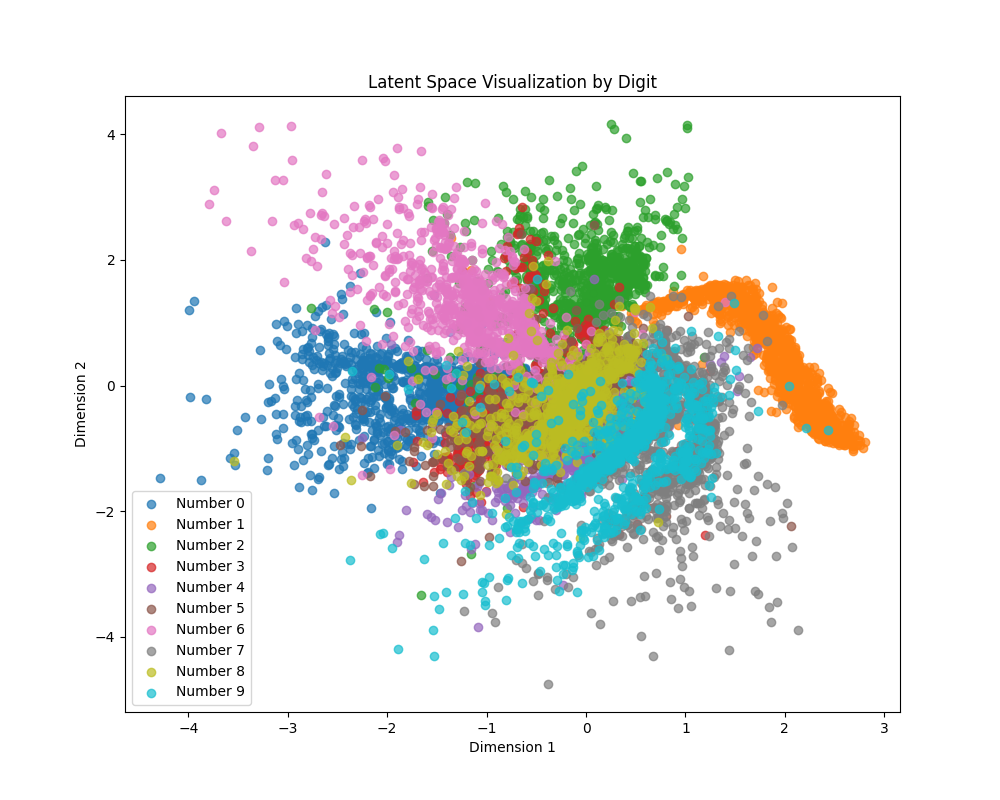
\includegraphics[width=0.6\textwidth]{images/latent_space_beta10.png}}
    \subfigure[Latent space for \(\beta = 30\)]{
    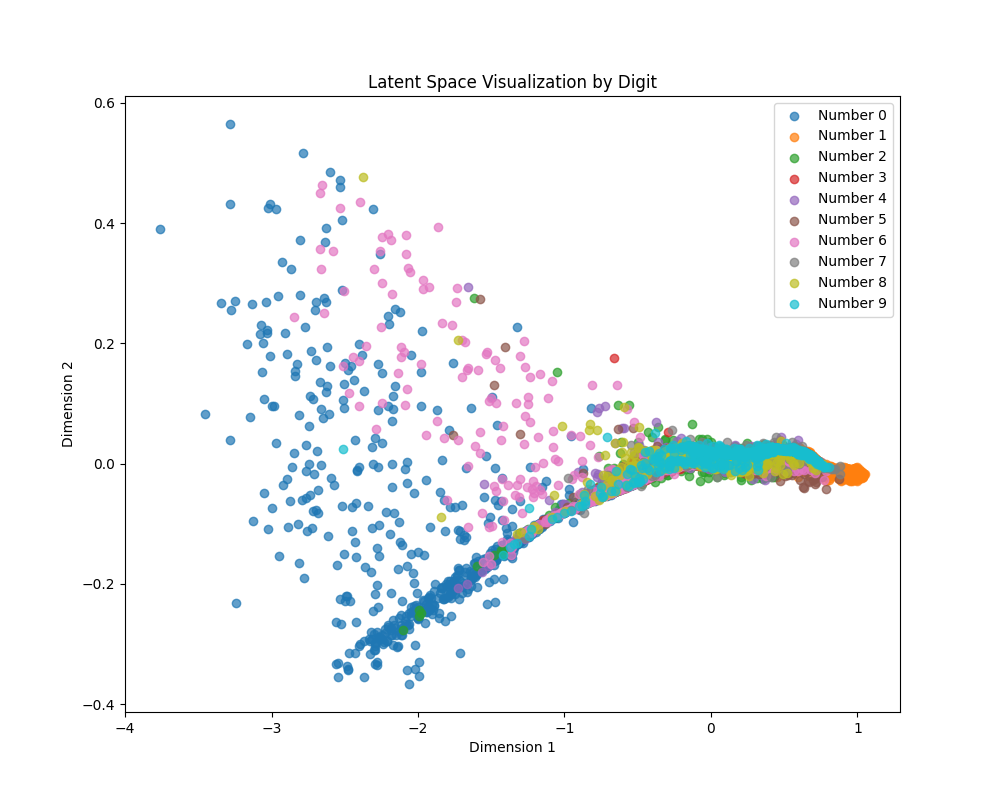
\includegraphics[width=0.6\textwidth]{images/latent_space_beta30.png}}
    \caption{2-dimensional latent spaces for different values of \(\beta\)}
    \label{latentbeta2d}
\end{figure}

In Figure \ref{latentbeta2d} we can clearly notice why the generated images of each model come out in their particular form. While the \(\beta = 10\) model has a condensed but not too restricted latent space, the latent space of \(\beta = 30\) is highly condensed in a small region, making the random vectors that fall outside it an average of the images in the dataset. On the other hand we can see how \(\beta = 30\) generates well the number 0, which is just the distribution that spans most of the latent space. 

This behaviour is in agreement with the explanation we gave in Task 3.2 when the KL is too low, where the model reconstructs average images of the dataset (Figure \ref{recbeta2d}) where the KL values are very small. In addition, we can note for \(\beta = 10\) how the reconstructions also slightly improved the ones of Task 3.2 using less epochs.

\begin{figure}[H]
    \centering
    \subfigure[Reconstructions for \(\beta = 10\)]{
    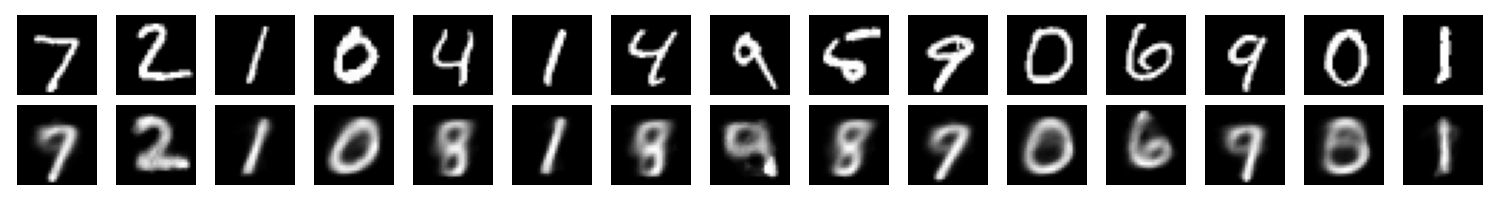
\includegraphics[width=0.6\textwidth]{images/reconstruction_beta10.png}}
    \subfigure[Reconstructions for \(\beta = 30\)]{
    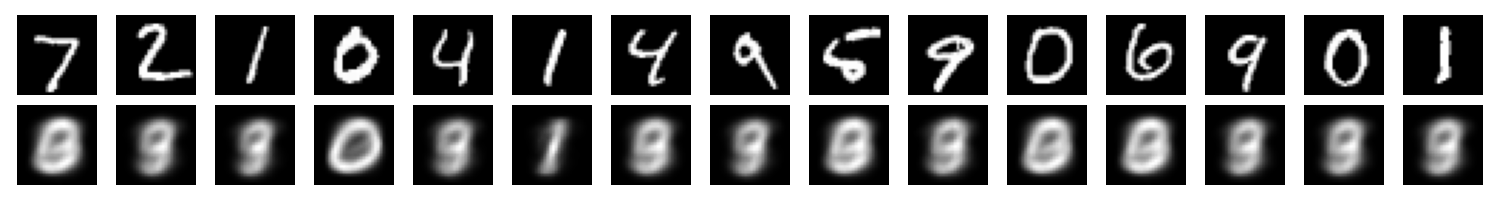
\includegraphics[width=0.6\textwidth]{images/reconstruction_beta30.png}}
    \subfigure[Likelihood and KL loss for \(\beta = 30\)]{
    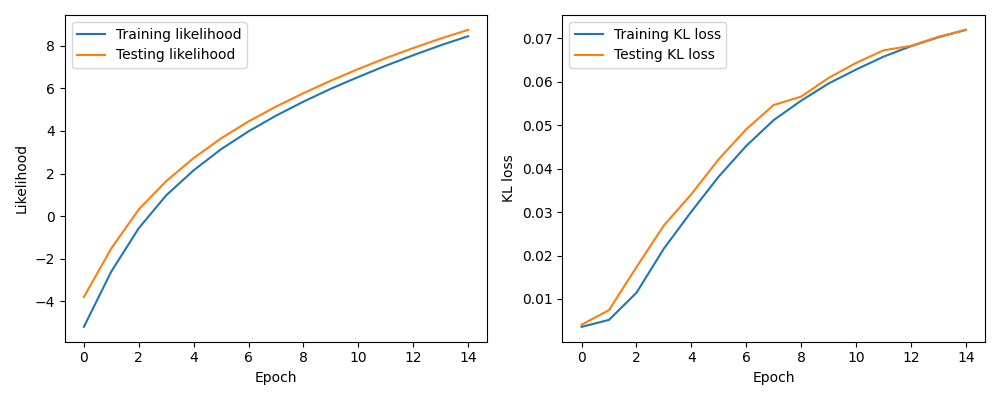
\includegraphics[width=0.6\textwidth]{images/likelihood_and_kl_loss_32_beta10.png}}
    \caption{Reconstructions for different values of \(\beta\)}
    \label{recbeta2d}
\end{figure}

\paragraph{\(\beta\) testing for 32-dimensional VAE} The 32-dimensional VAE output the best reconstructions but the generated digits were very bad. Now, we try to generate better images for this model.

We tried again with \(\beta = 10\) as it worked well in the 2-dimensional model.
\begin{figure}[H]
    \centering
    \subfigure[Generated images for \(\beta = 1\)]{
    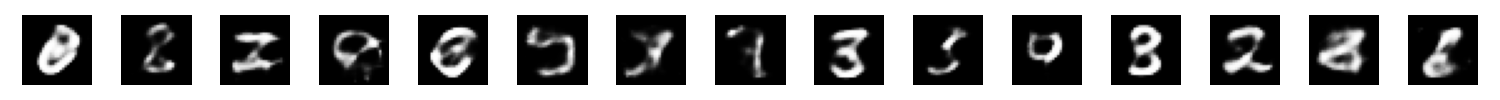
\includegraphics[width=0.6\textwidth]{images/generated_samples_25_32.png}}
    \subfigure[Generated images for \(\beta = 10\)]{
    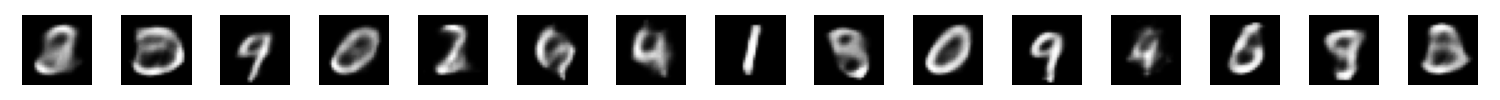
\includegraphics[width=0.6\textwidth]{images/generated_samples_32_beta10.png}}
    \caption{Comparison of generated images with the 32-dimensional model}
    \label{generated32beta}
\end{figure}

As we can observe in Figure \ref{generated32beta} the generated images are slightly better and clearer with \(\beta = 10\). However, the reconstruction gets a little more  and less detailed when constraining the latent space, as we can see in Figure \ref{rec32dbeta}. As we know, this happens because each number cloud is condensed together, making reconstruction more difficult but making it more likely that a random latent vector will have a detailed image associated with it (Figure \ref{latent32beta}).

\begin{figure}[H]
    \centering
    \subfigure[Reconstructed images for \(\beta = 1\)]{
    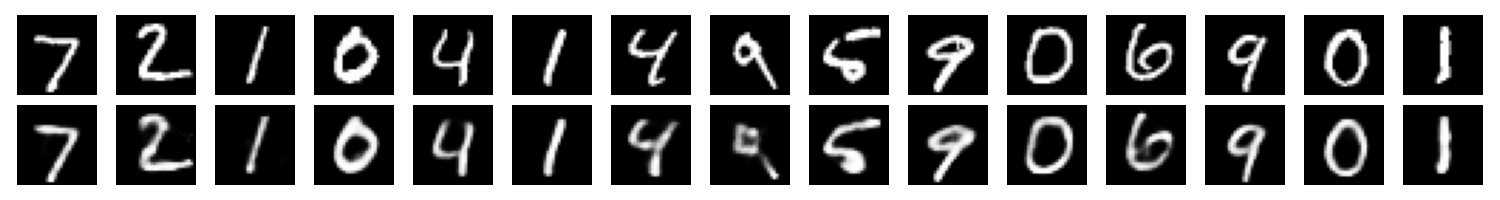
\includegraphics[width=0.6\textwidth]{images/reconstruction_25_32.png}}
    \subfigure[Reconstructed images for \(\beta = 10\)]{
    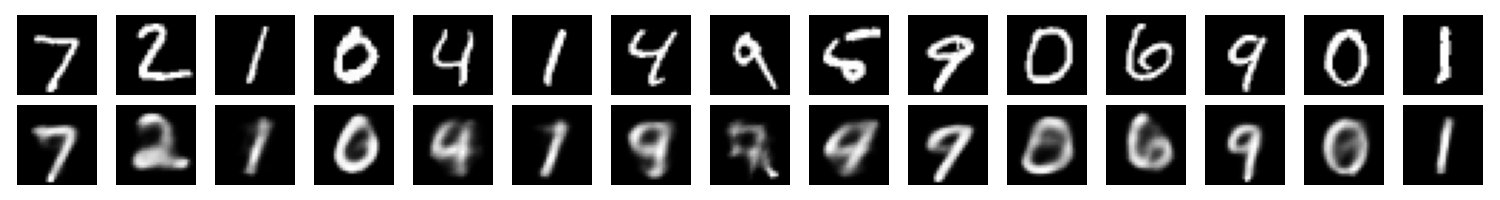
\includegraphics[width=0.6\textwidth]{images/reconstruction_32_beta10.png}}
    \caption{Comparison of reconstructed images with the 32-dimensional model}
    \label{rec32dbeta}
\end{figure}

\begin{figure}[H]
    \centering
    \subfigure[2d projection of latent space]{
    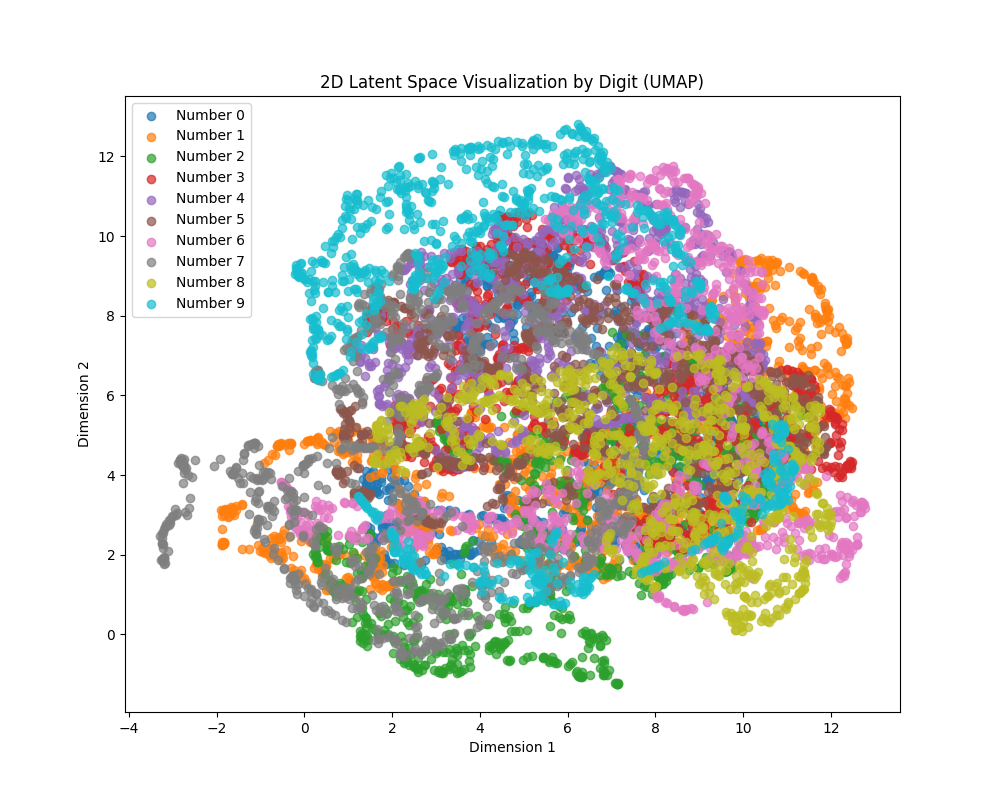
\includegraphics[width=0.6\textwidth]{images/latent_space_umap_32_beta10.png}}
    \subfigure[3d projection of latent space]{
    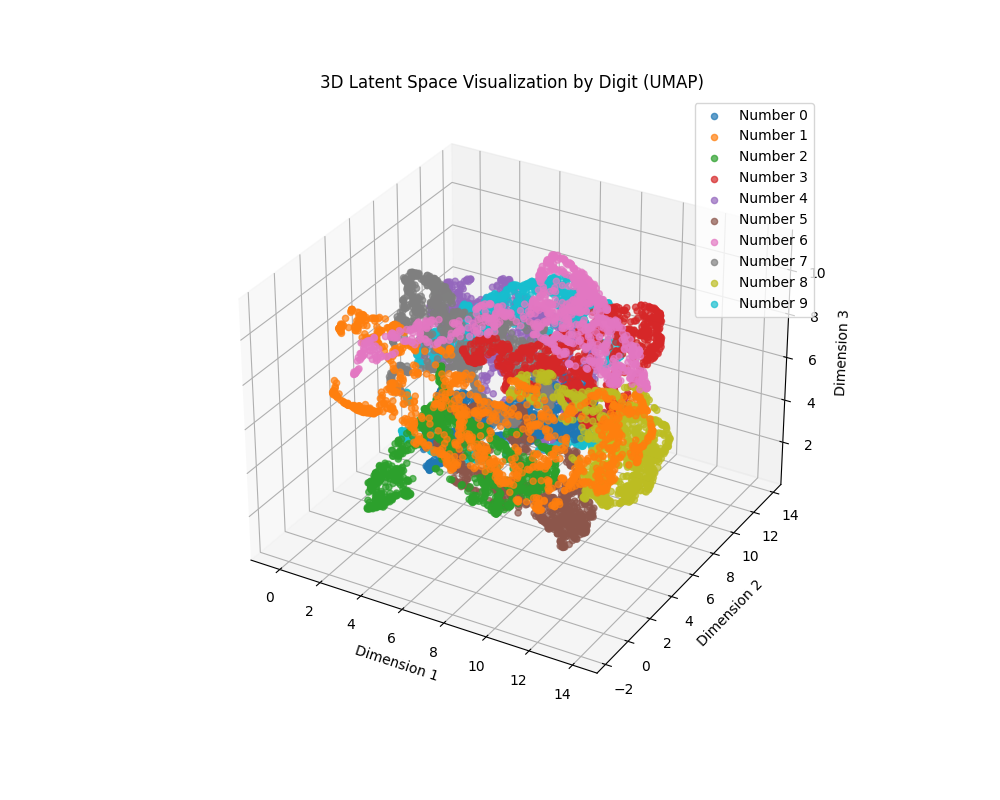
\includegraphics[width=0.7\textwidth]{images/latent_space_umap_3d_32_beta10.png}}
    \caption{UMAP reduction of the 32-dimensional space for\(\beta = 10\)}
    \label{latent32beta}
\end{figure}

Finally, we have explored the effects of adding the \(\beta\) parameter to the loss function that allows to apply more force to the KL regularization, producing a trade-off between reconstruction and generation making the latent space more or less similar to the prior distribution.


\paragraph{Answering the three questions from the first page of the exercise sheet}
\begin{itemize}
    \item (a) an estimate on how long it took you to implement and test the method. About 30h. The model last 1 minute per epoch so the accumulate time of testing is high.
    \item (b) how accurate you could represent data and what measure of accuracy you used. For the 2-dimensional VAE we got average reconstructions and generations. For the 32-dimensional VAE we got very detailed reconstructions but worse generated images. Finally we use the \(\beta\) parameter to get better generated images in the 2-dimensional and 32-dimensional model but at the expense of loosing reconstruction quality. As measures we used the likelihood of the reconstruction compared to the original image, as well as the Kl loss as an indicator of the latent space's structure. However, as we were working with images, we could use our own eyesight to discern whether reconstruction and generation were working well. Also, looking at the latent space representation we could infer if the model was working correctly.
    \item (c) what you learned about both the data set and the method (which is probably different from what the machine learned). We learned that the dataset was not as simple as it could seem. This can be shown when you need more than 2 latent dimensions to reconstruct the detailed image, because all the information in the image could not be reduced to 2 dimensions without losing part of it. Also, it was interesting to note the importance of the latent space structure in the performance of reconstructions and generations. Using the \(\beta\) parameter we could experiment with the trade-off between the performance on both quantities by manipulating the latent space structure, allowing us to understand better which structure benefits reconstructions and which one benefits generations.
\end{itemize}

\end{task}